% !TEX encoding = UTF-8 Unicode
\section{Indoor-Lokalisierung}

In dieser Ausarbeitung wird die Indoor-Lokalisierung von Personen betrachtet. Lokalisierung von Objekten ist ebenfalls denkbar, jedoch werden in den heutzutage verwendeten Systeme hauptsächlich Personen lokalisiert. Im Folgenden werden die Begriffe der \textit{aktiven Lokalisierung} und \textit{passiven Lokalisierung} eingeführt und kurz erläutert.

\subsection{Aktive Lokalisierung}
Unter einer \textit{aktiven Lokaliserung} versteht man Lokalisierungsmethoden, welche eine aktive Mitwirkung der Teilnehmer benötigt. Zumeist bedeutet dabei eine aktive Mitwirkung das Tragen eines Gerätes, welches mit den Sensoren im Raum in einer bestimmten Art und Weise kommuniziert.\footnote{Vgl. Deak G.,  Curran K. \& Condell J., S. 1}\\
Solche Systeme sind weit verbreitet, jedoch können Teilnehmer in manchen Situationen keine Gerätschaften bei sich tragen. Ein Beispiel dafür wäre eine Brandsituation. Die Einsatzkräfte der Feuerwehr würden mit aktiven Lokalisierungsmethoden im Regelfall nicht die Opfer ausfindig machen können, was im schlimmsten Fall Menschenleben kosten könnte.\\
Darüber hinaus können Personen selbst kleinste sichtbare Sensoren als unkomfortabel empfinden, sodass in solchen Situationen zu \textit{passiven Lokalisierungsmethoden} gegriffen werden muss.\footnote{Vgl. Kivimäki T., Vuorela T., Peltola P. \& Vanhala J., S.1}
\subsection{Passive Lokalisierung}
Im Gegensatz zur \textit{aktiven Lokalisierungsmethoden} wird bei einer \textit{passiven Lokalisierung} (auch \textit{sensorlose Lokalisierung}) keine aktive Mitwirkung der Teilnehmer verlangt.\footnote{Vgl. ebd.} Ein großer Vorteil solcher Systeme ist die Benutzerfreundlichkeit, da keinerlei Gerätschaften sich am Teilnehmer selbst befinden müssen. Ebenfalls bieten \textit{sensorlose Lokaliserungsmethoden} neue Anwendungsbereiche wie zum Beispiel Alarmanlagen in Gebäuden. So können Einbrecher lokalisiert werden, was bei \textit{aktiver Lokalisierung} nur schwer vorstellbar ist.\\
Die folgende Abbildung zeigt nochmals die Unterkategorien von \textit{Indoor-Lokalisierung} auf:

\begin{figure}[H]
	\centering
	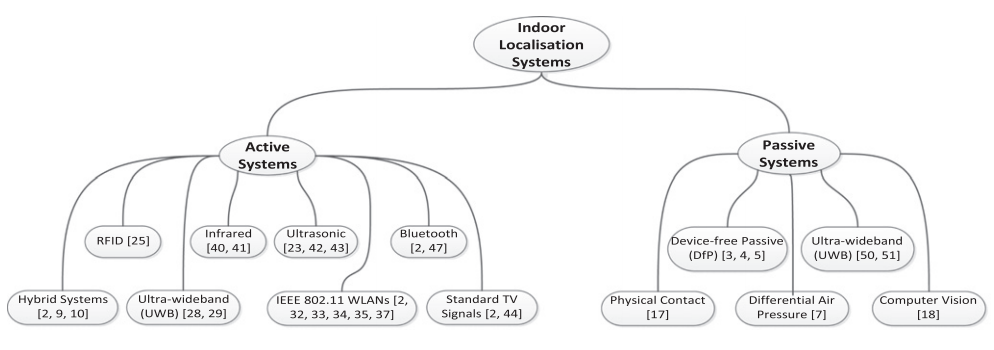
\includegraphics[scale=0.9]{pictures/indoor_loc}
	\caption{Unterkategorien von Indoor-Lokalisierung (Deak G.,  Curran K. \& Condell J., S. 2)}
\end{figure}

Im weiteren Verlauf wird jedes \textit{passive System} näher untersucht. Es wird die Funktionsweise sowie die Vor- und Nachteile des jeweiligen Systems erläutert.


\section{Sensorlose Indoor-Lokalisierung}
\subsection{Radiosignale}
\subsubsection{Radio Frequency Identification}
Unter \textit{Radio Frequence Identification} (\textbf{RFID}) versteht man eine kontaktlose Identifikation mittels Funkübertragung. Oftmals kann man hierfür bereits vorhandene Wi-Fi-Netzwerke verwenden.\footnote{Vgl. Kivimäki T., Vuorela T., Peltola P. \& Vanhala J., S.  16} \\
Ein solches DfL-System (\textbf{Device-free Localization}) nutzt die Tatsache aus, dass die Präsenz eines menschlichen Körpers die Radiosignale beeinflusst.\footnote{Vgl. ebd.} Die verwendete Frequenz der Knotenpunkte liegt hierbei bei $2.4$Ghz, weil dies die Resonanzfrequenz von Wasser ist und der Mensch bekanntermaßen aus $70\%$ aus Wasser besteht.\footnote{Vgl. Deak G.,  Curran K. \& Condell J., S. 11}. Ein weiterer Pluspunkt ist auch, dass die Frequenz von $2.4$ Ghz bei \textit{IEEE Standards} wie $802.11b$ und $802.11g$ verwendet wird.\footnote{Vgl. Pirzada N.,Nayan Y., Subhan F., Hassan F., Khan M., S. 3}\\
Das \textit{DfP-System} (\textit{Device-free Passive}) auf Grundlage von \textit{RFID}, welches im Folgenden vorgestellt wird, misst die Änderungen von der erhaltenen \textit{Received Signal Strength Indication} (\textbf{RSSI}). Der Anwendungsbereich des vorgestellten Systems ist die Haussicherheit. Das System soll als Alarmanlage agieren und Eindringlinge lokalisieren bzw. detektieren können.\footnote{Vgl. Mah M., S. 2} Ein solches System besteht aus zwei Komponenten, den \textit{Access Points} (\textbf{AP})\footnote{Z. Dt. Zugriffsknoten} und den \textit{Monitoring Points} (\textbf{MP})\footnote{(Z. Dt. Kontrollknoten)}. Einen guten Überblick bietet die folgende Abbildung:\\

\begin{figure}[H]
	\centering
	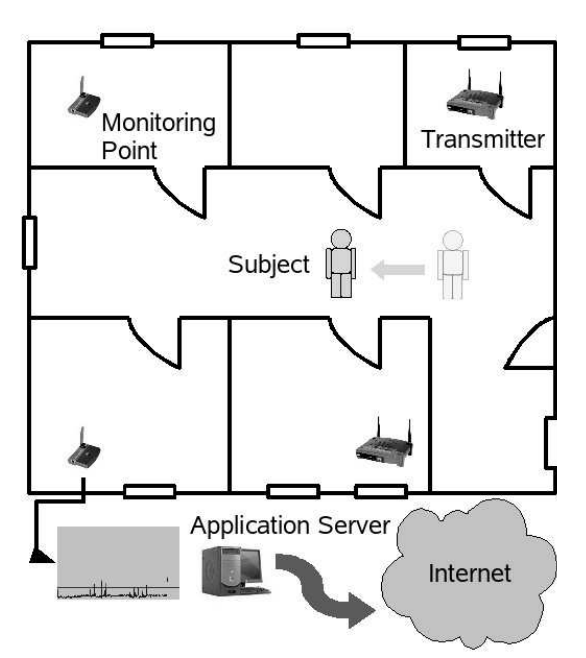
\includegraphics[width=0.5\textwidth]{pictures/rfid}
	\caption{RFID Indoor-Lokalisierung (Matthew Mah, S. 2)}
\end{figure}

In der obigen Abbildung erkennt man zwei \textbf{AP}, sowie einen \textbf{MP} und einen \textbf{DfP Server}, der die Berechnungen auf Grundlage der erhaltenen Signale durchführt. Als \textbf{MP} können dabei beliebige Computer verwendet werden.\footnote{Vgl. ebd.} Neben der eigentlichen Detektion (\textit{Monitoring Mode}) unterstützt das System noch zwei weitere Modi, welche nun näher beschrieben werden.\\

\begin{itemize}
\item \textbf{Monitoring Mode}: Dieser Modus nimmt jegliche Aktivität wahr, eignet sich somit für eine nächtliche Überwachung.
\item \textbf{Tracking mode}: Dieser Modus kann einen Eindringling orten und zusätzlich noch anhand der Daten der, die von den \textbf{MP} verzeichnet werden, verfolgen. Es kann nur ein Eindringling zu einem bestimmten Zeitpunkt geortet werden.
\item \textbf{DfP Mode}: Der \textit{DfP-Modus} kann mehrere Eindringlinge gleichzeitig orten und verfolgen.
\end{itemize}

Sobald ein Eindringling von einem \textbf{MP} detektiert wird, werden zusätzlich noch weitere \textit{Monitoring Points} kontaktiert und auf mögliche Detektionen überprüft. Erst danach kommt es zu einem Alarm des Gesamtsystems.\footnote{Vgl. ebd., S. 2 f.} Tests in kontrollierten Umgebungen ergaben zufriedenstellende Ergebnisse mit einer niedrigen Rate von \textit{False Positives}\footnote{Z. Dt. Falschpositiv} und einer hohen \textit{Detektionsrate}. Die beiden beiden folgenden Abbildungen zeigen dies nochmals graphisch auf.

\begin{figure}
\centering
\begin{minipage}{.5\textwidth}
  \centering
  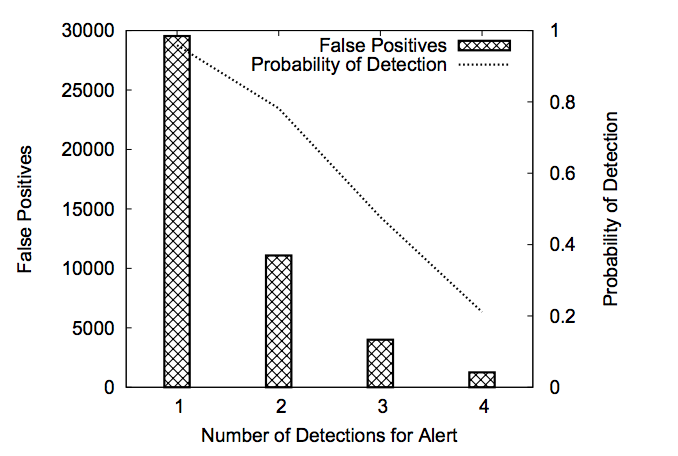
\includegraphics[scale=0.6]{pictures/false_pos}
  \caption*{False Positives}
\end{minipage}%
\begin{minipage}{.5\textwidth}
  \centering
  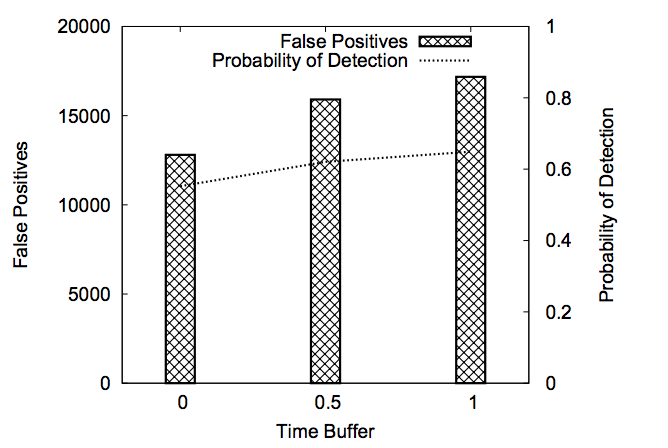
\includegraphics[scale=0.6]{pictures/detection}
  \caption*{Detection Rate}
\end{minipage}
\caption{Testergebnisse (Mah M., S. 9)}
\end{figure}

Dieses \textit{DfP-System} schnitt in den Tests zufriedenstellend ab, jedoch muss man auch auf mögliche Schwachstellen eingehen. Viele Parameter, die in den Algorithmen für die Detektion von Eindringlingen gebraucht werden haben direkten Einfluss auf die Sensibilität des Systems. Will man die Wahrscheinlichkeit eine Detektion zu verzeichnen erhöhen, wird gleichzeitig die Anzahl der \textit{False Positives} erhöht. Das Finden von Parametern, welche die Wahrscheinlichkeit von Detektionen erhöhen und gleichzeitig die Anzahl der \textit{False Positives} minimieren, ist ein Optimierungsproblem.\footnote{Vgl. ebd. S. 9}

\subsubsection{Ultra-wideband}

\textit{Ultra-wideband}\footnote{Z. Dt. Ultrabreitband} (\textbf{UWB}) ist eine weitere Methode Objekte zu lokalisieren. Bei \textbf{UWB} werden sehr große Frequenzbereiche zur Nahbereichskommunikation verwendet. Dabei werden vier Arten von UWB-Imaging\footnote{Z. Dt. Darstellung} unterschieden:\footnote{Vgl. Deak G.,  Curran K. \& Condell J., S. 12}
\begin{itemize}
 	\item \textbf{Ground Penetrating Radar}: Detektion vergrabener Objekte 
 	\item \textbf{Wall Imaging}: Detektion von Objekten innerhalb dichter Wände
 	\item \textbf{Through-wall Imaging}: Detektion von Objekten oder Personen auf der anderen Seite einer Wand
 	\item \textbf{Medical Imaging}: Verwendung für medizinische Zwecke
 \end{itemize} 

Das erste System, was eine Überwachung durch Wände ermöglichte, verwendete Signale mit einer Frequenz zwischen $902$ und $928$ MHz. Dieses System war in der Lage sich bewegende Objekte mit bis zu $1.5$ $m/s$ zu detektieren. Wurde eine Bewegung detektiert, so wurde vom Empfänger ein akkustisches Signal ausgelöst. Der Nachteil dieses Systems war jedoch, dass das Signal Wände mit Spiegeln oder allgemein nasse Wände nur schlecht penetrieren konnte. Systeme, die hingegen auf \textbf{UWB} basieren, verwenden Frequenzen von $3.1$ bis $10.6$ GHz, die eine Penetration von Wänden ermöglichen. Darüber hinaus sind diese Systeme resistenter gegenüber Interferenz sowie Multipath-Fading\footnote{Z. Dt. Mehrwegempfang}\footnote{Vgl. ebd.} \\
\textbf{UWB}-Systeme beheben viele der Probleme, die bei \textit{Narrowband}-Systemen\footnote{Z. Dt. Schmalband} entstehen können, gleichzeitig gibt es, wie bei jedem System, aber auch Kehrseiten. Zwar wurden Experimente mit \textbf{UWB}-Lokalisierungssystemen durchgeführt, es gibt jedoch keine einheitlichen Methoden zur Detektion von Objekten und zur Verarbeitung der Signale. Ebenso muss in der Mehrheit der existierenden Systeme eine Lerndatenbank gepflegt werden, die erstellt werden muss bevor die eigentliche Lokalisierung vonstattengehen kann.\footnote{Vgl. Kilic Y., Wymeersch H., Meijerink A., Bentum M. \& Scanlon W., S. 1}\\
Abschließend kann man sagen, dass Systeme, die auf Radiosignalen basieren ihren Zweck erfüllen, es jedoch kein universelles System gibt und man je nach Einsatzgebiet ein passendes Verfahren auszuwählen hat.


\subsection{Passive Infrarot-Lokalisierung}
Die passive Infrarot-Lokalisierung (\textbf{PIL}) basiert auf der Körperwärmestrahlung einer Person bzw. eines Objektes. Der thermische Unterschied eines Objektes im Vergleich zu seiner Umgebung kann dabei zur Lokalisierung und Bewegungsverfolgung (Tracking) ausgenutzt werden. Die untere Abbildung zeigt die unterschiedliche Wärmestrahlung einer Person und gegenüber seiner Umgebung.

\begin{figure}[H]
	\centering
	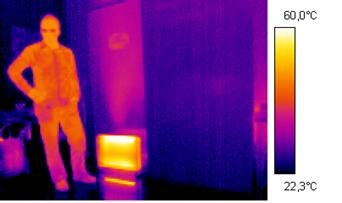
\includegraphics[width=0.5\textwidth]{pictures/pil1}
	\caption{Wärmestrahlung einer Person (Technische Universität Dortmund (2015))}
\end{figure}

Die Detektion der Wärmestrahlung wird durch sogenannte Thermopiles\footnote{Z.Dt. Thermosäulen}  realisiert.\footnote{Vgl. Technische Universität Dortmund 2015} Dabei handelt es sich um elektronische Bauelemente, welche thermische Energie in elektrische Energie umwandeln.\footnote{Vgl. Kemper 2010, S. 33} Um eine Person zu lokalisieren bzw. zu tracken, werden mehrere dieser Sensoren im Raum positioniert, um die thermischen Unterschiede zu messen. Auf Grundlage der so ermittelten Daten können anschließend mit Hilfe spezieller Algorithmen die Sichtwinkel auf die entsprechende Person berechnet werden. Durch Triangulation kann durch diese Winkel die Position eines Objektes bestimmt werden.\footnote{Vgl. Technische Universität Dortmund 2015} Die untere Abbildung skizziert dieses Verfahren.

\begin{figure}[H]
	\centering
	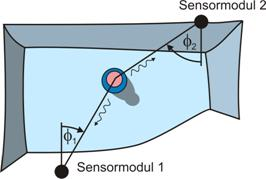
\includegraphics[width=0.5\textwidth]{pictures/triangulation}
	\caption{Lokalisierung durch Triangulation (Technische Universität Dortmund (2015))}
\end{figure}

Der Vorteil dieser Methode liegt nicht nur in der Tatsache, dass ein zu lokalisierendes Objekt keine zusätzliche Hardware mitführen muss. Durch den Verzicht bildgebender Sensoren wird zusätzlich ein Schutz der Privatsphäre gewährleistet.\footnote{Vgl. Kemper 2010, S. 149} Weiterhin ist diese Art der Lokalisierung gegenüber anderen Methoden vergleichsweise kostengünstig.\footnote{Vgl. Kemper 2010, S. 149}\footnote{Vgl. Deak G., Curran K. \& Condell J., S. 7}

\subsection{Drucksensoren}
\subsubsection{Bla}
\subsubsection{BlaBla}
\subsection{Computer-Vision}
Auch Computer-Vision kann als \textbf{DfP}-System betrachtet werden, da ein potentieller Nutzer keine zusätzliche Hardware am Körper tragen muss. Das Ziel dieses Systems ist, eine Umgebung zu schaffen, die auf die Position und das Verhalten einer Person reagiert (intelligente Umgebung). \footnote{Vgl. Deak G., Curran K. \& Condell J., S. 13}\newline Es ist beispielsweise vorstellbar, dass 

Test

\subsection{Fazit}

\subsection{Ausblick}

\newpage

\section{Quellenverzeichnis}
\subsection*{Literaturquellen}
\begin{itemize}[leftmargin=*]
\item[] \textbf{Sample}
\end{itemize}
\subsection*{Sonstige Quellen}
\begin{itemize}[leftmargin=*]
\item[] \textbf{Deak G., Curran K. \& Condell J.} A survey of active and passive indoor localisation systems (2012), Online unter URL : \url{http://scisweb.ulster.ac.uk/~kevin/comcomsurvey.pdf}
\item[] \textbf{Ehrlich, I.}: Indoor Localization (2006), Online unter URL: \url{http://ifgi.uni-muenster.de/~muellerj/lbs06/proceedings/3-IndoorLocalization.pdf}
\item[] \textbf{Kemper J.}: Passive Infrarot-Lokalisierung (2010), Fakultät für Elektrotechnik und Informationstechnik, Technischen Universität Dortmund, Dortmund
\item[] \textbf{Kilic Y., Wymeersch H., Meijerink A., Bentum M. \& Scanlon W.}: Online unter URL: \url{http://arxiv.org/pdf/1303.4092.pdf}
\item[] \textbf{Kivimäki T., Vuorela T., Peltola P. \& Vanhala J.}: A Review on Device-Free Passive Indoor Positioning Methods (2014), Online unter URL: \url{http://www.sersc.org/journals/IJSH/vol8_no1_2014/9.pdf}
\item[] \textbf{M. Mah}: Device-Free Passive Localization (2007), Online unter URL: \url{https://www.cs.umd.edu/sites/default/files/scholarly_papers/MatthewMah_1.pdf}
\item[] \textbf{Pirzada N.,Nayan Y., Subhan F., Hassan F., Khan M.}: Device-Free Localization Technique for Indoor Detection and Tracking of Human Body (2013), Online unter URL: \url{http://ac.els-cdn.com/S187704281402878X/1-s2.0-S187704281402878X-main.pdf?_tid=7bc6ad0e-12a4-11e5-95f4-00000aab0f02&acdnat=1434293516_4a2274a0ebfb932cf57c3f4f652c668f}
\item[] \textbf{Technische Universität Dortmund}: TU Dortmund, Fakultät ETIT, IRF, IT, Forschung, Embedded Systems,  Projekte, PIL, DFG-Projekt: Passive Infrarot-Lokalisierung, Online unter URL: \url{http://www.irf.tu-dortmund.de/cms/de/IT/Forschung/Embedded_Systems/Projekte/PIL/index.html}, Abruf: 2015-06-15
\end{itemize}